\documentclass[a4paper]{article}
\usepackage[a4paper]{geometry}
\usepackage[utf8]{inputenc}
\usepackage{polski}
\usepackage[polish]{babel}
\usepackage[T1]{fontenc}
\usepackage{graphicx}
\usepackage{verbatim}
\usepackage{float}
\usepackage{minted}
\usepackage{microtype}
\usepackage{shortvrb}
\usepackage{amsmath}

\let\olditemize=\itemize \let\endolditemize=\enditemize \renewenvironment{itemize}{\olditemize \itemsep0em}{\endolditemize}

\title{TEMAT ĆWICZENIA: OpenGL – projekt systemu słonecznego}
\author{Marcel Guzik}

\begin{document}
\section{Wprowadzenie}

Celem ćwiczenia jest wykonanie projektu inkorporującego wszystkie techniki
OpenGL poznane podczas kursu, wykonując interaktywny model systemu słonecznego.

\begin{figure}[H]
      \centering
      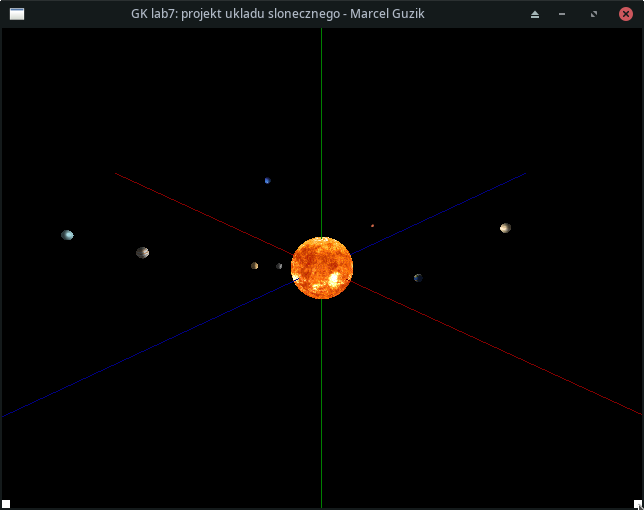
\includegraphics[width=0.3\textwidth]{img/1}
      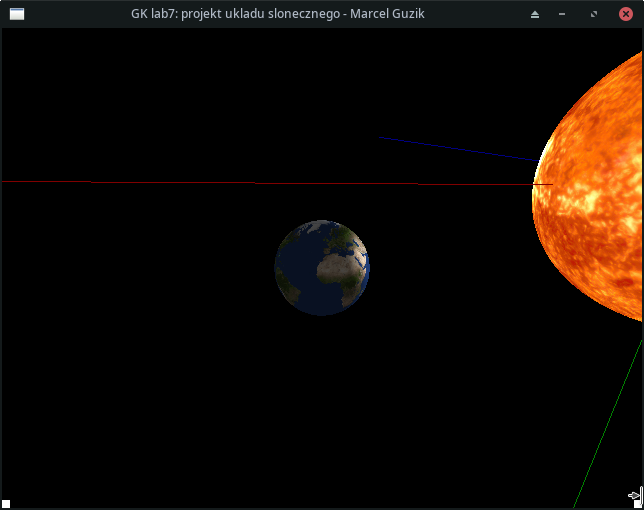
\includegraphics[width=0.3\textwidth]{img/2}
      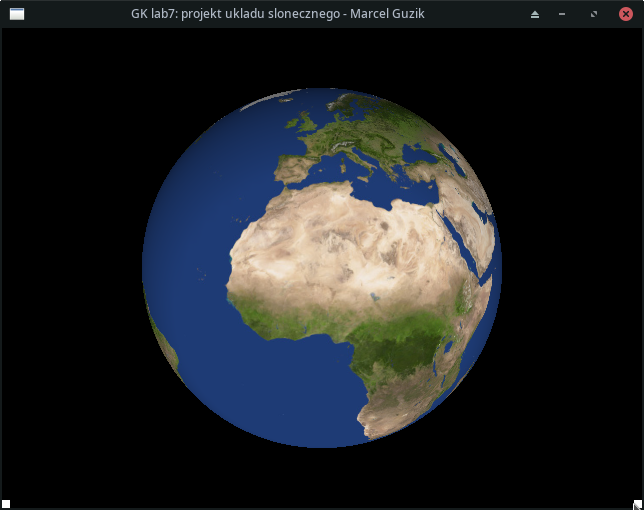
\includegraphics[width=0.3\textwidth]{img/3}
      \caption{Kopie widoku okna programu przedstawiające słońce, planety układu
            słonecznego oraz zbliżenie na Ziemię}
\end{figure}

\section{Zakres projektu}

Zaimplementowano:

\begin{itemize}
      \item Realistyczny system oświetlenia przez oświetlanie i cieniowanie
            Phonga
      \item Intuicyjne sterowanie kamerą
      \item Poruszanie planetami wg. ich orbit dookoła słońca, które dla
            uproszczenia w programie są idealnymi okręgami
      \item Kontrolę czasu by przyśpieszać lub spowalniać obieg planet.
\end{itemize}

Nie zaimplementowano:

Symulowane są tylko główne planety systemu słonecznego, bez ich naturalnych
satelitów. Skala wielkości planet oraz odległości między nimi nie są
realistyczne i zostały wybrane arbitralnie by zagwarantować poglądowość modelu.
Model symuluje rotację planet wokół słońca, wokół własnej osi Y, jednak nie mają
inklinacji orbity (wszystkie poruszają się na tej samej powierzchni) ani
pochylenia osiowego, rotacja wokół własnej osi wszystkich planet jest w tym
samym kierunku.

\section{Kod programu}

\inputminted[breaklines]{C}{../main.cpp}

\section{Podsumowanie}

Wykonany program skupił w sobie techniki poznane w trakcie kursu Grafika
Komputerowa. Wykonany model systemu słonecznego zawiera jednak wiele uproszczeń.

\end{document}
